\section{Analyse et Pré-traitement des Données}
Dans un premier temps, les données d'entraînement (\textit{allocine\_genres\_train.csv}) peuvent être chargées grâce à la fonction \textsf{read\_csv} de la bibliotèque Pandas \cite{pandas} en précisant le séparateur (\textsf{sep=","}). L'utilisation des méthodes \textsf{head}, \textsf{tail}, \textsf{describe}, \textsf{info} et \textsf{hist} permettent de visualiser et comprendre les données contenues dans le jeu de données complet.

Dans le cadre de ce projet seules les données contenues dans les colonnes \textit{titre} et \textit{synopsis} seront utilisées pour déduire la valeur contenue dans \textit{genre}. Le jeu de données peut être réduit à ces trois features.\\
Etant donné que les données vont être utilisées pour de l'apprentissage automatique, il faut vérifier s'il y a des valeurs manquantes. Les méthodes \textsf{isna} et \textsf{sum} ne révèlent aucune valeur manquante dans les données d'entraînement.\\
La proportion des classes dans le jeu de données peut avoir un impact sur l'apprentissage. Les classes ayant un effectif plus faible seront généralement moins bien "apprises". La figure \ref{value_counts} montre que les classes n'ont pas toutes la même proportion dans le jeu de données: il y a beaucoup d'individus de la catégorie \textit{drame} alors que les classes \textit{biopic}, \textit{documentaire} et \textit{historique} sont très peu représentées.

\begin{figure}
    \center
    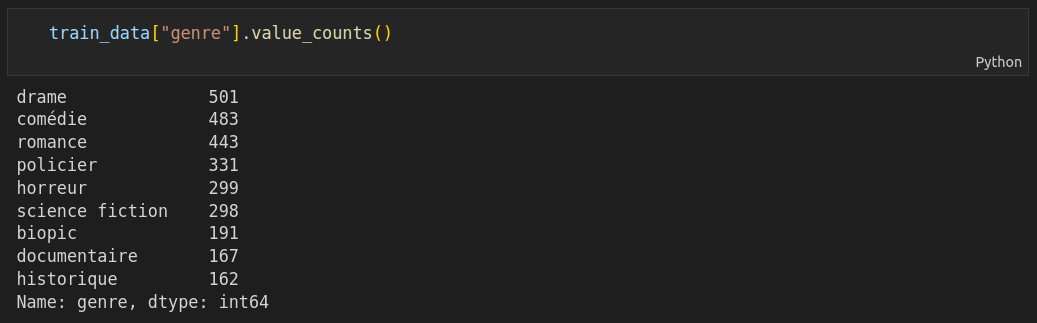
\includegraphics[scale=.3]{img/value_counts.png}
    \caption{Effectifs des classes dans les données d'entraînement}
    \label{value_counts}
\end{figure}

Après de nombreuses expériences, il s'avère que rééquilibrer les classes par \textit{oversampling}, c'est à dire: dupliquer des individus des classes les moins représentées, donne de meilleurs résultats quelque soit la méthode utilisée. \ref{confusion}\\
\textbf{Dans tout la suite,} les résultats présentés correpondront aux résultats obtenus avec le jeu de données d'entraînement rééquilibré par \textit{oversampling} à l'aide de l'objet \textsf{RandomOverSampler} de la bibliotèque Imbalanced-learn \cite{imbalanced_learn}.

\begin{figure}
    \centering
    \subfloat[\centering Matrice de confusion du modèle de régression logistique avec des classes déséquilibrées]{{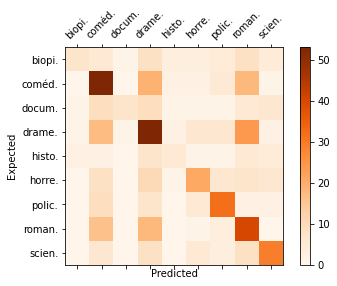
\includegraphics[width=5cm]{img/imbalanced.png}}}
    \qquad
    \subfloat[\centering Matrice de confusion du modèle de régression logistique avec des classes équilibrées par oversampling]{{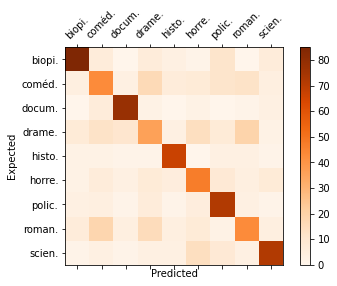
\includegraphics[width=5cm]{img/balanced.png}}}
    \caption{Comparaison des matrices de confusion pour des données déséquilibrées et équilibrées: les classes les moins représentées dans le jeu de données d'entraînement sont moins bien apprises lorsque les classes sont déséquilibrées.}
    \label{confusion}
\end{figure}

\noindent
\begin{minipage}[!hc]{0.12\textwidth}
   \textbf{Remarque}
\end{minipage}
\vrule\enskip\vrule\quad\begin{minipage}{\dimexpr 0.87\textwidth-0.8pt-1.5em}
Le jeu de données d'entraînement contient trop peu de données pour effectuer un équilibrage des classes par \textit{undersampling}, c'est à dire: supprimer des individus des classes les plus représentées. Les résultats obtenus avec cette méthode étaient généralement moins bons que sans équilibrage.
\end{minipage}